\documentclass[fr]{../../../../../../eplexam}

\graphicspath{{img/}}

\hypertitle{Mécanique des sols}{5}{GCIV}{1072}{2020}{Janvier}{Majeure}
{Michel-Antoine Fouarge}
{Henri de Chaunac}

\section{Questions de théorie}

\subsection{Question 1 (6 pts)}

Décrivez l'essai triaxial en conditions non-consolidé, non-drainé. Pourquoi obtient-on que $\phi' = 0$ ? 

\subsection{Question 2 (4 pts)}

Démontrez l'expression du facteur de sécurité pour la stabilité au glissement d'un sol non-drainé sur une pente inclinée.

\subsection{Question 3 (6 pts)}

Expliquer les 5 modes de rupture à vérifier lors du dimensionnnement d'un mur poids. Pour chaque mode de rupture, produire au moins un schéma, expliquer le calcul et donner une inégalité à vérifier. 

\subsection{Question 4 (4 pts)}

Expliquer de manière succinte (i.e. place limitée à 1/4 de feuille) : 

\begin{itemize}
	\item Pôle d'un cercle de Mohr
	\item État plan de déformation
	\item Tassement différentiel
	\item Critical State Line
\end{itemize}

\nosolution


\section{Exercices}

\subsection{Exercice 1 (3 pts)}

Justifier lequel de ces sols tassera plus vite ou plus lentement, en sachant qu'ils ont le même coefficient de compressibilité et qu'ils sont entourées par des couches qui sont soit perméables, soit imperméables. 

\begin{center}
    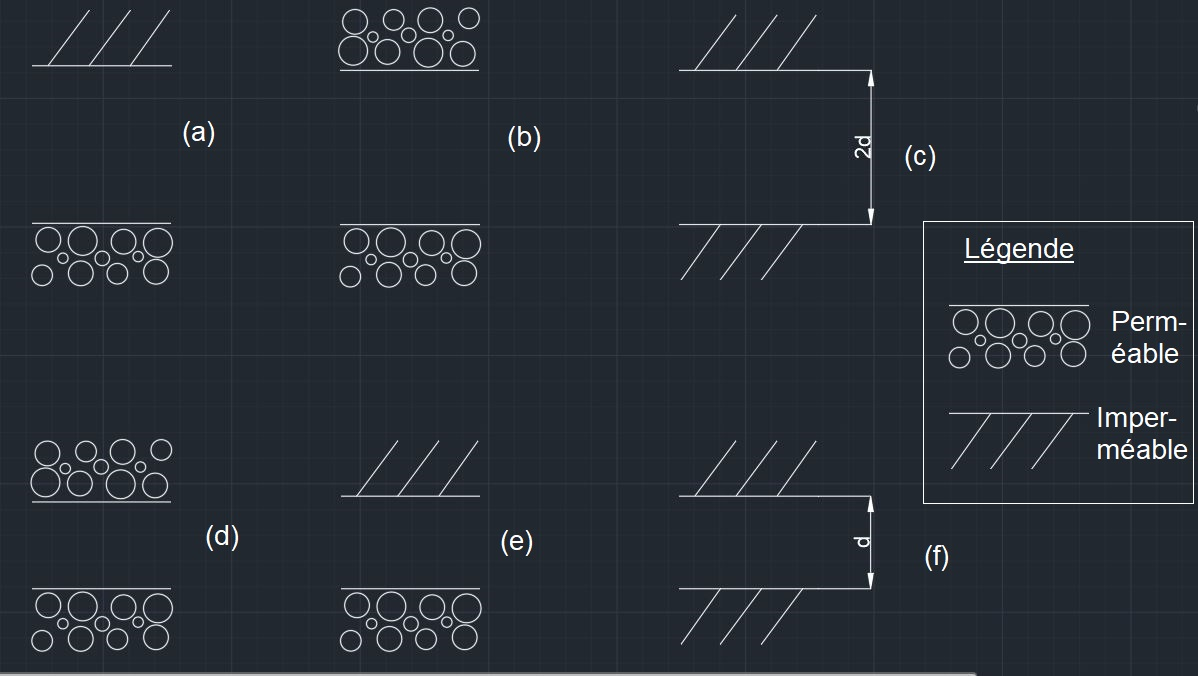
\includegraphics[scale = 0.5]{sols.jpg}
\end{center}

\subsection{Exercice 2 (2 pts)}

Sur base de l'abaque de Newton, quelle pente permet d'avoir un facteur de sécurité au glissement de 1,5 pour le talus ci-dessous ? 

\begin{center}
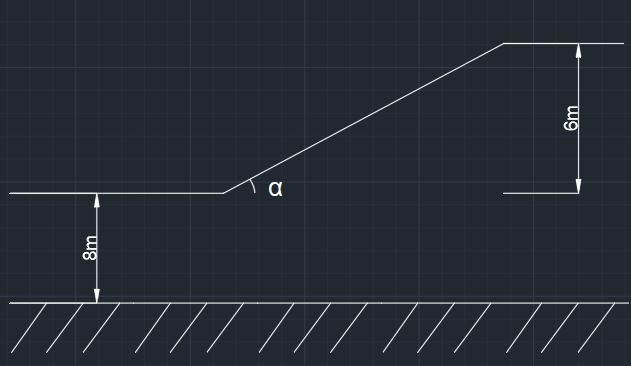
\includegraphics[scale=1]{Pente.jpg}
\end{center}

\subsection{Exercice 3 (5 pts)}

Nous disposons des résulatas de 3 essais effectués sur un sol.

\begin{itemize}
	\item Que vaut u pour le 3è essai
	\item Donner les valeurs de la cohésion c' et de l'angle de frottement $\phi'$
	\item En déduire u  pour le 2è essai
\end{itemize}

\begin{center}
\begin{tabular}{|cccc|}
	\hline
	Condition & $\sigma_1$ & $\sigma_1 - \sigma_3$ & u\\
	\hline
	UU & 100 & 50 & 40\\
	UU & 400 & 150 & ?\\
	CD & 400 & 250 & ?\\
	\hline
\end{tabular}
\end{center}

\subsection{Exercice 4 (3 pts)}

Semelle à 2m de profondeur. Quel côté b pour que sa base carrée aie un facteur de sécurité au poinçonnement  de 1,5 ($\phi'$ = 20°, c' = 80 kPa) ? 

\subsection{Exercice 5 (2 pts)}

On souhaite construire un tank circulaire de 20 mètres de diamètres sur un sol constitué d'une argile normalement consolidée ($C_c = 0,32$, $e_0 = 0,6$, $\gamma = 18 \frac{kN}{m^3}$). Calculer le tassement total sous le centre du tank en considérant une surcharge de 150 $\frac{kN}{m^2}$ et 5 couches de 4 mètres d'épaisseur.

\subsection{Exercice 6 (5 pts)}

On souhaite dimensionner un mur de soutènement à la pression latérale des terres, et à une surcharge répartie en surface de 50 kPa. 

\begin{center}
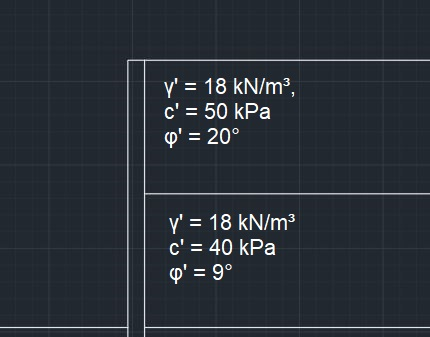
\includegraphics[scale=1]{Mur.jpg}
\end{center}

\begin{itemize}
	\item Dessiner le diagramme des pressions horizontales : pression $q_1$ due aux 4 premiers mètres de terres, $q_2$ due aux 4 autres mètres, et $q_s$ due à la surcharge.
	\item Calculer les forces $F_1$, $F_2$, et $F_s$ correspondantes.
	\item Calculer la force totale et son point d'application. 
	\item Refaire le calcul, pour une surcharge surfacique d'intensité nulle. 
\end{itemize}

\nosolution

\end{document}
